% =====================================================================
% Fluid Dynamics and IBM Theory: turbulence closure, RANS, LES, and hybrid methods
% =====================================================================
\documentclass[aspectratio=169,11pt]{beamer}

% Shared style, ported from the UF Animal Sciences 2026 talk (ib-tutorials.sty at the repo root).
\makeatletter\def\input@path{{./}{../}}\makeatother
\usepackage{ib-tutorials}

\usepackage[utf8]{inputenc}
\usepackage{amsmath,amssymb,bm,mathtools}
\usepackage{booktabs}
\usepackage{array}
\usepackage{xcolor}
\usepackage{tikz}
\usetikzlibrary{arrows.meta,calc,positioning,patterns,decorations.pathmorphing}
\usepackage{tcolorbox}
\tcbuselibrary{skins}
\usepackage{hyperref}

% Figure hues, mapped onto the muted talk palette.
\colorlet{modelblue}{NavyBlue!70}
\colorlet{modelorange}{orange!80!black}
\colorlet{modelgreen}{OliveGreen}
\colorlet{modelgray}{DarkGray}

\newcommand{\mean}[1]{\overline{#1}}
\newcommand{\Rey}{\mathrm{Re}}
\newcommand{\uu}{\bm{u}}
\newcommand{\xvec}{\bm{x}}
\newcolumntype{L}[1]{>{\raggedright\arraybackslash}p{#1}}
% The title slide uses \maketutorialtitlepanel{...} from ib-tutorials.sty,
% which places arbitrary content (here a TikZ sketch) in the right-hand column.

\title[Turbulence closure]{Turbulence closure: RANS, LES, and hybrid ideas}
\subtitle{What is averaged, what is filtered, and what must be modeled?}
\author[Miller]{Laura A. Miller}
\institute[UArizona]{Department of Mathematics, University of Arizona}
\date{Fluid Dynamics and IBM Theory \textbullet\ Module 5\\[3pt]
  Adapted in part from lectures by Steven L. Brunton; equations follow Pope (2000) and Wilcox (2006).}

\begin{document}

% ----- 1. Title -----
\begin{frame}[plain]
\maketutorialtitlepanel{%
    \begin{punchbox}
    \centering
    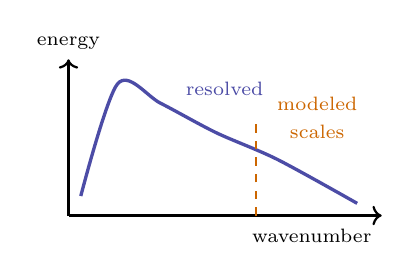
\begin{tikzpicture}[x=0.78cm,y=0.62cm]
      \draw[->,thick] (0,0)--(5.1,0) node[below left=1pt and 0pt]{\scriptsize wavenumber};
      \draw[->,thick] (0,0)--(0,3.2) node[above]{\scriptsize energy};
      \draw[very thick,modelblue] plot[smooth] coordinates{(0.2,0.4)(0.8,2.7)(1.5,2.3)(2.4,1.7)(3.4,1.15)(4.7,0.25)};
      \draw[dashed,modelorange,thick] (3.05,0)--(3.05,2.0);
      \node[modelblue,anchor=west] at (1.75,2.6){\scriptsize resolved};
      \node[modelorange,align=center] at (4.05,2.0){\scriptsize modeled\\[-2pt]\scriptsize scales};
    \end{tikzpicture}
    \end{punchbox}}
\end{frame}

% ----- 2. Why model? -----
\begin{frame}{Why turbulence modeling?}
\begin{columns}[T,onlytextwidth]
\begin{column}{0.52\textwidth}
Engineering design asks for quantities such as
\begin{itemize}\itemsep4pt
  \item lift, drag, stall, and wall loading;
  \item wake recovery, mixing, heat transfer, and noise;
  \item performance over \emph{many} geometries and operating points.
\end{itemize}
\begin{block}{The modeling bargain}
Spend fewer degrees of freedom on the smallest motions, but retain the physics needed for the chosen quantity of interest.
\end{block}
\end{column}
\begin{column}{0.45\textwidth}
\centering
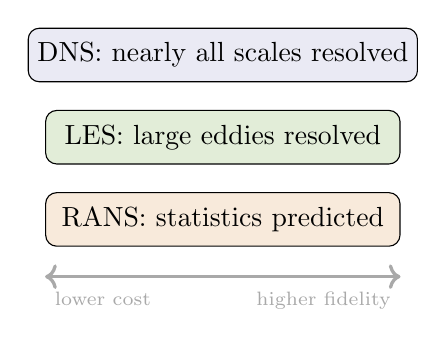
\begin{tikzpicture}[node distance=0.35cm]
  \node[draw,rounded corners,fill=modelblue!12,minimum width=4.5cm,minimum height=0.68cm] (dns) {DNS: nearly all scales resolved};
  \node[draw,rounded corners,fill=modelgreen!12,below=of dns,minimum width=4.5cm,minimum height=0.68cm] (les) {LES: large eddies resolved};
  \node[draw,rounded corners,fill=modelorange!14,below=of les,minimum width=4.5cm,minimum height=0.68cm] (rans) {RANS: statistics predicted};
  \draw[<->,very thick,modelgray] ([yshift=-0.38cm]rans.south west)--([yshift=-0.38cm]rans.south east);
  \node[anchor=north west,modelgray] at ([yshift=-0.45cm]rans.south west){\scriptsize lower cost};
  \node[anchor=north east,modelgray] at ([yshift=-0.45cm]rans.south east){\scriptsize higher fidelity};
\end{tikzpicture}
\vspace{0.5em}

\soft{No method is ``best'' without a flow, grid, wall treatment, and target output.}
\end{column}
\end{columns}
\end{frame}

% ----- 3. DNS cost -----
\begin{frame}{DNS resolves the cascade---at a steep cost}
\begin{columns}[T,onlytextwidth]
\begin{column}{0.52\textwidth}
DNS advances the Navier--Stokes equations without a turbulence closure and resolves down to the dissipative scales.

For idealized three-dimensional turbulence,
\[
  \frac{\eta}{L}\sim \Rey_L^{-3/4},
  \qquad
  N_{\mathrm{grid}}\sim \left(\frac{L}{\eta}\right)^3\sim \Rey_L^{9/4}.
\]
The time-step count also grows as the smallest time scale shrinks.

\begin{block}{Interpret the scaling carefully}
It is an order-of-magnitude argument, not a universal cost law for every geometry or numerical method.
\end{block}
\end{column}
\begin{column}{0.45\textwidth}
\centering
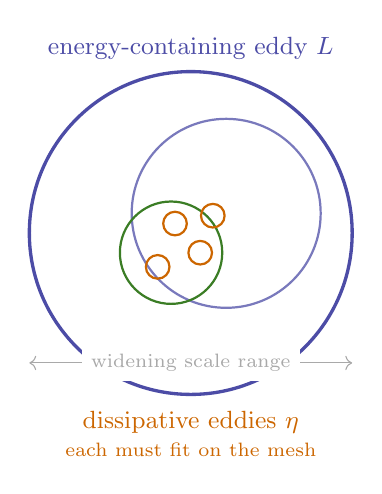
\begin{tikzpicture}
  \draw[very thick,modelblue] (0,0) circle (2.05);
  \draw[thick,modelblue!75] (0.45,0.25) circle (1.20);
  \draw[thick,modelgreen] (-0.25,-0.25) circle (0.65);
  \foreach \x/\y in {-0.20/0.12,0.12/-0.25,0.28/0.22,-0.42/-0.43}{
    \draw[modelorange,thick] (\x,\y) circle (0.15);
  }
  \node[modelblue] at (0,2.35){\small energy-containing eddy $L$};
  \node[modelorange,align=center] at (0,-2.55){\small dissipative eddies $\eta$\\[-2pt]\scriptsize each must fit on the mesh};
  \draw[<->,modelgray] (-2.05,-1.65)--(2.05,-1.65) node[midway,fill=white]{\scriptsize widening scale range};
\end{tikzpicture}
\end{column}
\end{columns}
\end{frame}

% ----- 4. Goal -----
\begin{frame}{Choose the fidelity that answers the question}
\small
\setlength{\tabcolsep}{3pt}
\begin{tabular}{@{}L{0.16\textwidth}L{0.23\textwidth}L{0.25\textwidth}L{0.23\textwidth}@{}}
\toprule
\textbf{Method} & \textbf{Directly computed} & \textbf{Modeled} & \textbf{Typical role}\\
\midrule
DNS & all dynamically relevant velocity scales & no turbulence closure & canonical flows; reference data\\[3pt]
LES & filtered, unsteady large scales & subfilter stress; often wall effects & wakes, mixing, separated unsteadiness\\[3pt]
RANS/URANS & mean or phase-resolved mean field & all turbulent correlations & design sweeps; attached wall flows\\[3pt]
Hybrid RANS--LES & RANS region plus resolved eddies elsewhere & region- and grid-dependent & high-$\Rey$ separated flows\\
\bottomrule
\end{tabular}

\vspace{0.6em}
\begin{punchbox}
\centering
\hi{Closure} means representing terms created by averaging or filtering that are not determined by the retained variables.
\end{punchbox}
\end{frame}

% ----- 5. Reynolds averaging -----
\begin{frame}{RANS begins with an averaging operator}
For velocity and kinematic pressure,
\[
  u_i(\xvec,t)=U_i(\xvec,t)+u_i'(\xvec,t),
  \qquad
  p=P+p',
  \qquad
  \mean{u_i'}=\mean{p'}=0.
\]
Here $U_i=\mean{u_i}$ may be an ensemble, long-time, or statistically equivalent average.

\begin{columns}[T,onlytextwidth]
\begin{column}{0.48\textwidth}
\begin{block}{Steady RANS}
For statistically stationary flow, a long-time mean is independent of time: $\partial_t U_i=0$.
\end{block}
\end{column}
\begin{column}{0.48\textwidth}
\begin{block}{URANS}
Retain $\partial_t U_i$ when the chosen mean is time dependent; modeled turbulence still lies beneath that mean.
\end{block}
\end{column}
\end{columns}

For incompressible constant-density flow, $\partial_i U_i=0$ and $\partial_i u_i'=0$.
\end{frame}

% ----- 6. RANS equation -----
\begin{frame}{Averaging creates the Reynolds-stress divergence}
With pressure normalized by density, the incompressible RANS/URANS equations are
\begin{align*}
  \partial_t U_i+U_j\partial_jU_i
  &= -\partial_iP+\nu\partial_{jj}U_i-\partial_jR_{ij},\\
  \partial_iU_i&=0,
  \qquad R_{ij}:=\mean{u_i'u_j'}.
\end{align*}

\begin{punchbox}
\centering
The physical turbulent stress is $-\rho R_{ij}$; the equation contains $-\partial_jR_{ij}$.
The sign convention must remain paired with the closure.
\end{punchbox}
\vspace{0.8em}

\begin{columns}[t,onlytextwidth]
\begin{column}{0.48\textwidth}
$R_{ij}$ is symmetric and positive semidefinite.
\end{column}
\begin{column}{0.48\textwidth}
$R_{ii}=2k$ fixes its trace through the TKE.
\end{column}
\end{columns}
\end{frame}

% ----- 7. Hierarchy -----
\begin{frame}{Why not derive an exact equation for $R_{ij}$?}
\centering
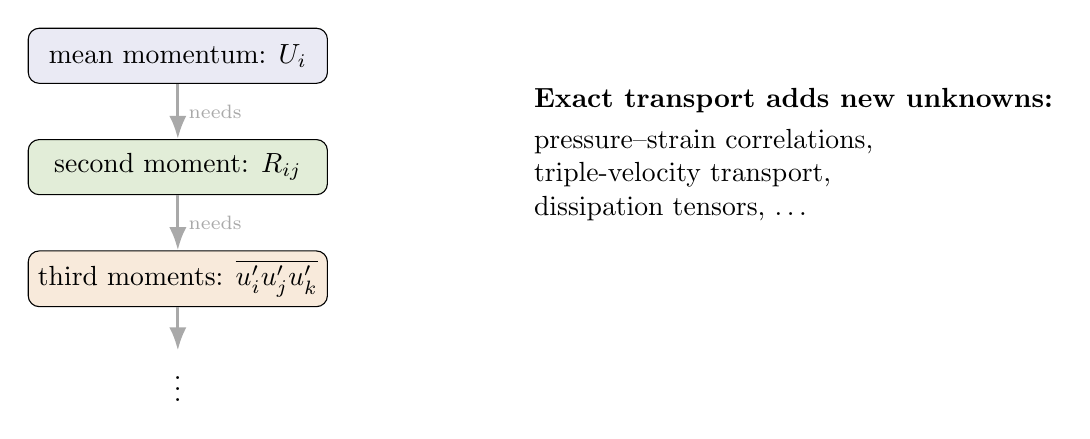
\begin{tikzpicture}[node distance=0.7cm,>=Latex]
  \node[draw,rounded corners,fill=modelblue!12,minimum width=3.8cm,minimum height=0.7cm] (mean) {mean momentum: $U_i$};
  \node[draw,rounded corners,fill=modelgreen!12,below=of mean,minimum width=3.8cm,minimum height=0.7cm] (second) {second moment: $R_{ij}$};
  \node[draw,rounded corners,fill=modelorange!14,below=of second,minimum width=3.8cm,minimum height=0.7cm] (third) {third moments: $\mean{u_i'u_j'u_k'}$};
  \node[below=0.55cm of third] (dots) {$\vdots$};
  \draw[->,very thick,modelgray] (mean)--(second) node[midway,right]{\scriptsize needs};
  \draw[->,very thick,modelgray] (second)--(third) node[midway,right]{\scriptsize needs};
  \draw[->,very thick,modelgray] (third)--(dots);
  \node[align=left,anchor=west] at (4.4,-1.25) {\textbf{Exact transport adds new unknowns:}\\[3pt]
    pressure--strain correlations,\\
    triple-velocity transport,\\
    dissipation tensors, $\ldots$};
\end{tikzpicture}

\vspace{0.7em}
\begin{block}{Closure is structural, not a bookkeeping nuisance}
Moment equations form a hierarchy: an assumption, modeled equation, or data-driven relation is needed to stop it.
\end{block}
\end{frame}

% ----- 8. TKE -----
\begin{frame}{Turbulent kinetic energy condenses the normal stresses}
\[
  k:=\frac12R_{ii}
  =\frac12\left(\mean{u'^2}+\mean{v'^2}+\mean{w'^2}\right).
\]

\begin{columns}[T,onlytextwidth]
\begin{column}{0.49\textwidth}
\begin{block}{What $k$ measures}
Fluctuation kinetic energy per unit mass. It is nonnegative and has units $L^2/T^2$.
\end{block}
\end{column}
\begin{column}{0.47\textwidth}
\begin{block}{What $k$ does not determine}
The scalar $k$ fixes only $\mathrm{tr}(R)$; it does not determine stress anisotropy or shear stresses.
\end{block}
\end{column}
\end{columns}

\vspace{0.5em}
\hi{Modeling lens:} follow how mean-flow energy becomes turbulent energy, moves through space and scale, and is dissipated by viscosity.
\end{frame}

% ----- 9. TKE budget -----
\begin{frame}{The exact TKE budget names the competing processes}
For incompressible, constant-property flow,
\[
  \partial_tk+U_j\partial_jk
  =\underbrace{-R_{ij}\partial_jU_i}_{\mathcal P}
   -\underbrace{\varepsilon}_{\ge 0}
   -\partial_jT_j,
\]
\[
  \varepsilon=\nu\mean{\partial_ju_i'\,\partial_ju_i'},
  \qquad
  T_j=\tfrac12\mean{u_i'u_i'u_j'}+\mean{p'u_j'}-\nu\partial_jk.
\]
{\small This is the pseudo-dissipation; it differs from $2\nu\mean{s_{ij}'s_{ij}'}$ by a term that vanishes in homogeneous turbulence.}

\centering
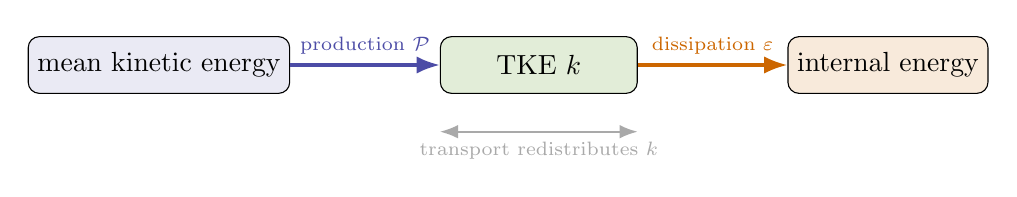
\begin{tikzpicture}[node distance=0.45cm,>=Latex]
  \node[draw,rounded corners,fill=modelblue!12,minimum width=2.5cm,minimum height=0.72cm] (mean) {mean kinetic energy};
  \node[draw,rounded corners,fill=modelgreen!12,right=1.9cm of mean,minimum width=2.5cm,minimum height=0.72cm] (tke) {TKE $k$};
  \node[draw,rounded corners,fill=modelorange!14,right=1.9cm of tke,minimum width=2.5cm,minimum height=0.72cm] (heat) {internal energy};
  \draw[->,very thick,modelblue] (mean)--(tke) node[midway,above]{\scriptsize production $\mathcal P$};
  \draw[->,very thick,modelorange] (tke)--(heat) node[midway,above]{\scriptsize dissipation $\varepsilon$};
  \draw[<->,thick,modelgray] ([yshift=-0.48cm]tke.south west)--([yshift=-0.48cm]tke.south east)
    node[midway,below]{\scriptsize transport redistributes $k$};
\end{tikzpicture}
\end{frame}

% ----- 10. Production -----
\begin{frame}{Production is a signed exchange with the mean flow}
Because $R_{ij}$ is symmetric,
\[
  \mathcal P=-R_{ij}\partial_jU_i=-R_{ij}S_{ij},
  \qquad
  S_{ij}=\tfrac12(\partial_jU_i+\partial_iU_j).
\]

For a parallel shear flow $U=(U(y),0,0)$,
\[
  \mathcal P=-\mean{u'v'}\,\frac{\mathrm dU}{\mathrm dy}.
\]

\begin{columns}[T,onlytextwidth]
\begin{column}{0.49\textwidth}
\begin{block}{Common wall-flow signs}
$\mathrm dU/\mathrm dy>0$ and $\mean{u'v'}<0$ give $\mathcal P>0$: mean energy feeds turbulence.
\end{block}
\end{column}
\begin{column}{0.47\textwidth}
\begin{alertblock}{Do not infer the sign from ``separation''}
Separated shear often produces turbulence strongly, but local production can be negative.
\end{alertblock}
\end{column}
\end{columns}
\end{frame}

% ----- 11. Boussinesq -----
\begin{frame}{Boussinesq closes stress with a scalar eddy viscosity}
\begin{columns}[T,onlytextwidth]
\begin{column}{0.57\textwidth}
The linear eddy-viscosity hypothesis is
\[
  -R_{ij}=2\nu_tS_{ij}-\frac23k\delta_{ij},
\]
or equivalently $R_{ij}=\tfrac23k\delta_{ij}-2\nu_tS_{ij}$.

For incompressible flow, absorb the isotropic part into
\[
  P^*=P+\frac23k.
\]

\begin{block}{Modeling task}
Specify the scalar field $\nu_t\ge 0$ from algebra, auxiliary transport equations, or data.
\end{block}
\end{column}
\begin{column}{0.40\textwidth}
\centering
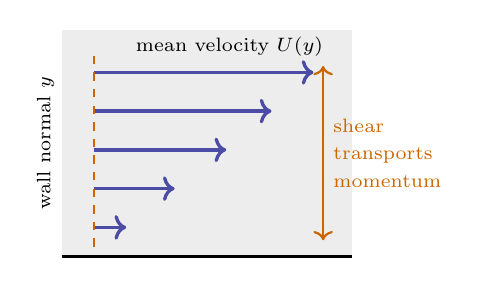
\begin{tikzpicture}[x=0.82cm,y=0.82cm]
  \fill[LightGray!40] (0,0) rectangle (4.5,3.5);
  \draw[very thick] (0,0)--(4.5,0);
  \draw[->,modelblue,very thick] (0.5,0.45)--(1.0,0.45);
  \draw[->,modelblue,very thick] (0.5,1.05)--(1.75,1.05);
  \draw[->,modelblue,very thick] (0.5,1.65)--(2.55,1.65);
  \draw[->,modelblue,very thick] (0.5,2.25)--(3.25,2.25);
  \draw[->,modelblue,very thick] (0.5,2.85)--(3.9,2.85);
  \draw[dashed,modelorange,thick] (0.5,0.15)--(0.5,3.15);
  \node[rotate=90] at (-0.25,1.75){\scriptsize wall normal $y$};
  \node at (2.6,3.25){\scriptsize mean velocity $U(y)$};
  \draw[<->,modelorange,thick] (4.05,0.25)--(4.05,2.95)
    node[midway,right,align=left]{\scriptsize shear\\[-2pt]\scriptsize transports\\[-2pt]\scriptsize momentum};
\end{tikzpicture}
\end{column}
\end{columns}
\end{frame}

% ----- 12. Constant eddy viscosity -----
\begin{frame}{Zero-equation baseline: constant $\nu_t$}
The simplest choice is
\[
  \nu_t=\text{constant},
  \qquad
  \nu_{\mathrm{eff}}=\nu+\nu_t.
\]

\begin{columns}[T,onlytextwidth]
\begin{column}{0.48\textwidth}
\begin{block}{Why keep this model?}
It exposes the mechanism, is inexpensive, and can be calibrated for a narrow configuration.
\end{block}
\end{column}
\begin{column}{0.48\textwidth}
\begin{alertblock}{Why it is not predictive}
One constant cannot represent wall damping, free-stream intermittency, spatially varying shear, or history effects.
\end{alertblock}
\end{column}
\end{columns}

\vspace{0.6em}
\hi{Useful baseline question:} which observed behavior can be explained by enhanced momentum diffusion alone?
\end{frame}

% ----- 13. Mixing length -----
\begin{frame}{Prandtl mixing length connects shear and momentum exchange}
\begin{columns}[T,onlytextwidth]
\begin{column}{0.56\textwidth}
For a parallel shear flow,
\[
  \nu_t=\ell_m^2\left|\frac{\mathrm dU}{\mathrm dy}\right|.
\]
The mixing length $\ell_m$ represents a displacement over which a fluid parcel retains velocity contrast.

\begin{itemize}\itemsep3pt
  \item In the logarithmic layer, $\ell_m\approx\kappa y$ with the von K\'arm\'an constant $\kappa\approx0.41$.
  \item Near the wall and outside that layer, damping and outer-length caps are needed.
  \item This algebraic form is not a general three-dimensional closure.
\end{itemize}
\end{column}
\begin{column}{0.41\textwidth}
\centering
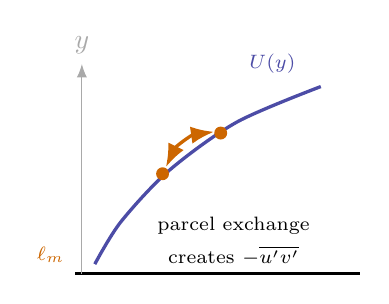
\begin{tikzpicture}[x=0.82cm,y=0.82cm,>=Latex]
  \draw[very thick] (0,0)--(4.4,0);
  \draw[modelblue,very thick] plot[smooth] coordinates{(0.3,0.15)(0.7,0.8)(1.45,1.6)(2.5,2.35)(3.8,2.9)};
  \node[modelblue] at (3.05,3.25){\scriptsize $U(y)$};
  \fill[modelorange] (1.35,1.55) circle (0.10);
  \fill[modelorange] (2.25,2.18) circle (0.10);
  \draw[<->,very thick,modelorange] (1.4,1.65) to[bend left=28] (2.15,2.2)
    node[midway,above left]{\scriptsize $\ell_m$};
  \draw[->,modelgray] (0.1,0)--(0.1,3.25) node[above]{$y$};
  \node[align=center] at (2.45,0.5){\scriptsize parcel exchange\\\scriptsize creates $-\mean{u'v'}$};
\end{tikzpicture}
\end{column}
\end{columns}
\end{frame}

% ----- 13b. Wall scaling and the log law -----
\begin{frame}{Wall scaling and the log law}
\begin{columns}[T,onlytextwidth]
\begin{column}{0.54\textwidth}
Wall units are built from the friction velocity:
\[
  u_\tau=\sqrt{\frac{\tau_w}{\rho}},
  \qquad
  y^+=\frac{y\,u_\tau}{\nu},
  \qquad
  U^+=\frac{U}{u_\tau}.
\]

\begin{itemize}\itemsep3pt
  \item \hi{Viscous sublayer:} $U^+=y^+$ for $y^+\lesssim5$.
  \item \hi{Log layer:} $U^+=\dfrac1\kappa\ln y^++B$ with $\kappa\approx0.41$ and $B\approx5.0$--$5.2$, for $30\lesssim y^+\lesssim0.1$--$0.2\,\delta^+$.
  \item \hi{Buffer layer} ($5\lesssim y^+\lesssim30$): neither law holds; turbulence production peaks near $y^+\approx12$.
\end{itemize}
{\scriptsize Here $\delta^+=\delta u_\tau/\nu$ is the friction Reynolds number; Pope (2000, Table~7.1) quotes the log law for $y^+>30$, $y/\delta<0.3$, and recent high-$\Rey$ data place its upper end nearer $0.15\,\delta$.\par}
\end{column}
\begin{column}{0.43\textwidth}
\centering
% Axes: s = ln y+ (x unit) and U+ (y unit), drawn to scale with kappa = 0.41, B = 5.2.
% On this semi-log axis the sublayer law U+ = y+ = e^s is a curve, the log law a line.
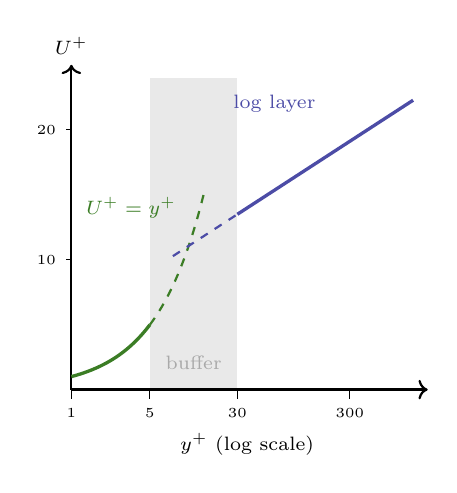
\begin{tikzpicture}[x=0.62cm,y=0.165cm]
  \fill[LightGray!50] ({ln(5)},0) rectangle ({ln(30)},24);
  \draw[->,thick] (0,0)--(7.3,0);
  \node[anchor=north] at (3.6,-2.6){\scriptsize $y^+$ (log scale)};
  \draw[->,thick] (0,0)--(0,25) node[above]{\scriptsize $U^+$};
  \foreach \yp/\lab in {1/1,5/5,30/30,300/300}{%
    \draw ({ln(\yp)},0)--({ln(\yp)},-0.7) node[below]{\tiny \lab};}
  \foreach \u in {10,20}{\draw (0,\u)--(-0.12,\u) node[left]{\tiny \u};}
  % viscous sublayer U+ = y+ (solid where valid, dashed beyond)
  \draw[modelgreen,very thick,domain=0:{ln(5)},samples=40] plot (\x,{exp(\x)});
  \draw[modelgreen,thick,dashed,domain={ln(5)}:{ln(15)},samples=30] plot (\x,{exp(\x)});
  % log law U+ = (1/0.41) ln y+ + 5.2 (solid where valid, dashed below y+ = 30)
  \draw[modelblue,very thick,domain={ln(30)}:7,samples=2] plot (\x,{\x/0.41+5.2});
  \draw[modelblue,thick,dashed,domain={ln(8)}:{ln(30)},samples=2] plot (\x,{\x/0.41+5.2});
  \node[modelgreen,anchor=west] at (0.1,14){\scriptsize $U^+=y^+$};
  \node[modelblue,anchor=east] at (5.2,22){\scriptsize log layer};
  \node[modelgray,anchor=south] at ({0.5*ln(150)},0.8){\scriptsize buffer};
\end{tikzpicture}

{\tiny\color{DarkGray} Drawn to scale ($\kappa=0.41$, $B=5.2$). Schematic: instructor's course notes, after Pope (2000), Ch.~7.\par}
\end{column}
\end{columns}
\end{frame}

% ----- 13c. Wall scaling in practice (split from the previous frame) -----
\begin{frame}{Wall scaling in practice: wall functions or wall resolution}
\begin{punchbox}
A \hi{wall function} imposes this profile at the first cell instead of resolving the sublayer, and needs the first cell centre near $30<y^+<300$. A \hi{low-$\Rey$} model instead resolves to $y^+\approx1$.
\end{punchbox}

\begin{itemize}\itemsep4pt
  \item $u_\tau$ is part of the solution, so a wall function solves the log law at the first cell for $u_\tau$ (and hence $\tau_w$) iteratively.
  \item Mesh design runs the other way: estimate $u_\tau$ from a skin-friction correlation, then place the first cell at $y=y^+\nu/u_\tau$.
  \item \hi{Worked example} (water, $\nu=10^{-6}\,\mathrm{m^2/s}$, $u_\tau=0.05$ m/s): $\nu/u_\tau=20\,\mu$m, so $y^+=1$ is $y=20\,\mu$m and $y^+=30$ is $y=0.6$ mm.
  \item A first cell in the buffer layer ($5\lesssim y^+\lesssim30$) satisfies neither approach; many codes then blend the two laws.
\end{itemize}
\end{frame}

% ----- 14. Two equation models -----
\begin{frame}{Two-equation models evolve turbulence scales}
\footnotesize
\setlength{\tabcolsep}{3pt}
\begin{tabular}{@{}L{0.18\textwidth}L{0.25\textwidth}L{0.20\textwidth}L{0.22\textwidth}@{}}
\toprule
\textbf{Family} & \textbf{Transported variables} & \textbf{Eddy viscosity} & \textbf{Key sensitivity}\\
\midrule
standard $k$--$\varepsilon$ & TKE $k$ and dissipation rate $\varepsilon$ & $\nu_t=C_\mu k^2/\varepsilon$ & near-wall treatment; separation\\[5pt]
$k$--$\omega$ & TKE $k$ and specific dissipation $\omega$ & $\nu_t=k/\omega$ (Wilcox) & free-stream $\omega$; practical limiters\\[5pt]
blended variants, e.g.\ Menter's SST $k$--$\omega$ (blending functions $F_1$, $F_2$ and a shear-stress limiter) & combine near-wall and outer-flow behavior & formulation dependent & calibration and blending functions\\
\bottomrule
\end{tabular}

\vspace{0.4em}
For the \emph{standard} $k$--$\varepsilon$ model, $C_\mu\approx0.09$ is a conventional empirical value; it is not universal across all variants.
The standard constants are $C_\mu=0.09$, $C_{\varepsilon1}=1.44$, $C_{\varepsilon2}=1.92$, $\sigma_k=1.0$, $\sigma_\varepsilon=1.3$ (Launder \& Spalding 1974).

\begin{punchbox}
Extra PDEs introduce memory, transport, and length/time scales---but they do not remove modeling assumptions.
\end{punchbox}
\end{frame}

% ----- 14b. The k-epsilon and k-omega transport equations -----
\begin{frame}{The $k$--$\varepsilon$ and $k$--$\omega$ transport equations}
\footnotesize
\begin{columns}[T,onlytextwidth]
\begin{column}{0.507\textwidth}
\hi{Standard $k$--$\varepsilon$} \soft{(Launder \& Spalding 1974)}
\begin{align*}
  \partial_t k + U_j\partial_j k &= P_k-\varepsilon
    +\partial_j\!\left[\left(\nu+\tfrac{\nu_t}{\sigma_k}\right)\partial_j k\right],\\
  \partial_t \varepsilon + U_j\partial_j \varepsilon &= C_{\varepsilon1}\frac{\varepsilon}{k}P_k
    -C_{\varepsilon2}\frac{\varepsilon^{2}}{k}
    +\partial_j\!\left[\left(\nu+\tfrac{\nu_t}{\sigma_\varepsilon}\right)\partial_j \varepsilon\right],
\end{align*}
\vspace{-1.1em}
\[
  \nu_t=C_\mu\frac{k^{2}}{\varepsilon}.
\]
\vspace{-1.0em}
\[
  P_k=-\mean{u_i'u_j'}\,\partial_j U_i=2\nu_t S_{ij}S_{ij}.
\]
\vspace{-0.6em}

Constants: $C_\mu=0.09$, $C_{\varepsilon1}=1.44$, $C_{\varepsilon2}=1.92$, $\sigma_k=1.0$, $\sigma_\varepsilon=1.3$.
\end{column}
\begin{column}{0.48\textwidth}
\hi{Wilcox $k$--$\omega$} \soft{(1988 form; the 2006 revision adds a cross-diffusion term and a stress limiter on $\nu_t$, and recalibrates the constants)}
\begin{align*}
  \partial_t k + U_j\partial_j k &= P_k-\beta^{*}k\omega
    +\partial_j\!\left[\left(\nu+\sigma_k\nu_t\right)\partial_j k\right],\\
  \partial_t \omega + U_j\partial_j \omega &= \alpha\frac{\omega}{k}P_k-\beta\omega^{2}
    +\partial_j\!\left[\left(\nu+\sigma_\omega\nu_t\right)\partial_j \omega\right],
\end{align*}
\vspace{-1.1em}
\[
  \nu_t=\frac{k}{\omega}.
\]
\vspace{-0.6em}

1988 constants: $\alpha=5/9$, $\beta=3/40$, $\beta^{*}=0.09$, $\sigma_k=\sigma_\omega=0.5$.

\soft{Note $\varepsilon\approx\beta^{*}k\omega$, so $\omega$ is a specific dissipation rate.}
\soft{(Wilcox defines $\omega=\varepsilon/(\beta^*k)$, so this holds by definition; diffusion coefficients multiply $\nu_t$ here but divide it in $k$--$\varepsilon$.)}
\end{column}
\end{columns}
\end{frame}

% ----- 14c. Near-wall behaviour (split from the previous frame) -----
\begin{frame}{Near-wall behaviour: why SST blends the two models}
\begin{punchbox}
$k$--$\varepsilon$ needs wall functions or damping terms near walls, because $\varepsilon$ does not behave well as $y\to0$ (at the wall $k\to0$ like $y^2$ while $\varepsilon$ stays finite, so the destruction term $C_{\varepsilon2}\varepsilon^2/k$ is singular and the model's near-wall $\nu_t$ is wrong without damping functions).\\[3pt]
$k$--$\omega$ integrates cleanly to the wall but is sensitive to the free-stream value of $\omega$---which is exactly why Menter's SST blends $k$--$\omega$ near the wall with $k$--$\varepsilon$ in the outer flow.
\end{punchbox}

\begin{itemize}\itemsep4pt
  \item Menter (1994) rewrites $k$--$\varepsilon$ in terms of $\omega$; the result is the $k$--$\omega$ equations plus a cross-diffusion term $2(1-F_1)\sigma_{\omega2}\,\omega^{-1}\partial_jk\,\partial_j\omega$.
  \item The blending function $F_1$ is $\approx1$ near the wall ($k$--$\omega$) and $\approx0$ in the outer layer and free stream ($k$--$\varepsilon$ behavior).
  \item The SST limiter $\nu_t=a_1k/\max(a_1\omega,\,\Omega F_2)$, $a_1=0.31$ ($\Omega$: vorticity magnitude; later versions use the strain rate $S$), caps the shear stress at $\approx a_1k$ (Bradshaw's assumption), improving adverse-pressure-gradient predictions.
\end{itemize}
\end{frame}

% ----- 15. SA -----
\begin{frame}{Spalart--Allmaras: a one-equation aerodynamic model}
\begin{columns}[T,onlytextwidth]
\begin{column}{0.58\textwidth}
SA transports a modified kinematic viscosity $\tilde\nu$ and reconstructs
\[
  \nu_t=\tilde\nu f_{v1}.
\]
Its transport equation balances production, diffusion, and near-wall destruction, with wall distance $d$ entering the model.

\begin{itemize}\itemsep3pt
  \item designed for aerodynamic, predominantly attached boundary layers;
  \item relatively economical and extensively used;
  \item behavior in separation, transition, rotation, and free shear depends on variant and setup.
\end{itemize}
\end{column}
\begin{column}{0.39\textwidth}
\centering
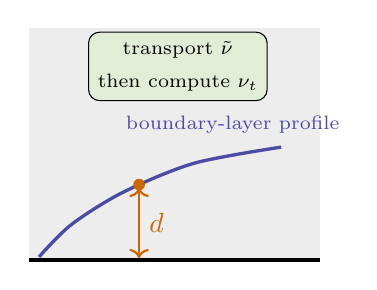
\begin{tikzpicture}[x=0.82cm,y=0.82cm]
  \fill[LightGray!40] (0,0) rectangle (4.5,3.6);
  \draw[very thick] (0,0)--(4.5,0);
  \draw[modelblue,very thick] plot[smooth] coordinates{(0.15,0.05)(0.65,0.55)(1.45,1.05)(2.55,1.5)(3.9,1.75)};
  \fill[modelorange] (1.7,1.17) circle (0.09);
  \draw[<->,modelorange,thick] (1.7,0.03)--(1.7,1.12) node[midway,right]{$d$};
  \node[modelblue] at (3.15,2.1){\scriptsize boundary-layer profile};
  \node[draw,rounded corners,fill=modelgreen!12,align=center] at (2.3,3.0){\scriptsize transport $\tilde\nu$\\\scriptsize then compute $\nu_t$};
\end{tikzpicture}

\vspace{0.35em}
{\scriptsize Model definition and variants: \href{https://tmbwg.github.io/turbmodels/spalart.html}{NASA Turbulence Modeling Resource}.\par}
\end{column}
\end{columns}
\end{frame}

% ----- 16. Separation -----
\begin{frame}{Separation exposes limits of scalar eddy viscosity}
\begin{columns}[T,onlytextwidth]
\begin{column}{0.50\textwidth}
Adverse pressure gradients can decelerate near-wall fluid, producing reversal and a recirculation region.

Linear eddy-viscosity models constrain stress anisotropy to align with the mean strain tensor. They may miss
\begin{itemize}\itemsep3pt
  \item anisotropy and curvature/rotation effects,
  \item nonequilibrium response and history,
  \item the onset and extent of separation.
\end{itemize}

\soft{This is a limitation of the closure class, not of Reynolds averaging itself.}
\end{column}
\begin{column}{0.47\textwidth}
\centering
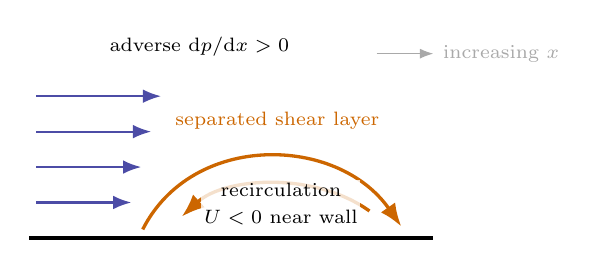
\begin{tikzpicture}[x=0.9cm,y=0.9cm,>=Latex]
  \draw[very thick] (0,0)--(5.7,0);
  \foreach \y in {0.5,1.0,1.5,2.0}{
    \draw[->,modelblue,thick] (0.1,\y)--(1.3+0.28*\y,\y);
  }
  \draw[modelorange,very thick,->] (1.6,0.12) .. controls (2.3,1.5) and (4.35,1.45) .. (5.25,0.16);
  \draw[modelorange,very thick,->] (4.8,0.38) .. controls (4.0,0.95) and (2.75,0.85) .. (2.15,0.3);
  \node[modelorange] at (3.5,1.65){\scriptsize separated shear layer};
  \node[align=center,fill=white,fill opacity=0.8,text opacity=1,inner sep=1pt] at (3.55,0.48){\scriptsize recirculation\\[-2pt]\scriptsize $U<0$ near wall};
  \draw[->,modelgray] (4.9,2.6)--(5.7,2.6) node[right]{\scriptsize increasing $x$};
  \node at (2.4,2.7){\scriptsize adverse $\mathrm dp/\mathrm dx>0$};
\end{tikzpicture}
\end{column}
\end{columns}
\end{frame}

% ----- 17. RANS checkpoint -----
\begin{frame}{RANS checkpoint: keep three layers distinct}
\begin{enumerate}\itemsep8pt
  \item \hi{Exact averaged equation:}
  $R_{ij}=\mean{u_i'u_j'}$ appears through $-\partial_jR_{ij}$.
  \item \hi{Constitutive hypothesis:}
  a scalar eddy viscosity sets $-R_{ij}^{\mathrm{dev}}=2\nu_tS_{ij}$.
  \item \hi{Model for $\nu_t$:}
  constant, mixing length, $k$--$\varepsilon$, $k$--$\omega$, SA, or another closure.
\end{enumerate}

\begin{punchbox}
\centering
Changing the equation for $\nu_t$ cannot repair every limitation imposed by the scalar Boussinesq relation.
\end{punchbox}
\end{frame}

% ----- 18. LES transition -----
\begin{frame}{LES asks a different question}
RANS asks: \emph{what are the statistics?}\\[3pt]
LES asks: \emph{which motions can this grid resolve, and how do the rest affect them?}

\vspace{0.6em}
\begin{columns}[T,onlytextwidth]
\begin{column}{0.48\textwidth}
\begin{block}{Resolve}
Large, geometry-dependent, energy-containing motions and their unsteady transport.
\end{block}
\end{column}
\begin{column}{0.48\textwidth}
\begin{block}{Model}
The effect of motions below the filter width, including energy transfer across the cutoff.
\end{block}
\end{column}
\end{columns}

\begin{alertblock}{Conditional advantage}
LES can improve predictions of wakes and separated unsteadiness only when grid resolution, numerics, inflow, SGS closure, and wall treatment are adequate.
\end{alertblock}
\end{frame}

% ----- 19. Filtering -----
\begin{frame}{Filtering is not Reynolds averaging}
Define a spatially filtered field by convolution,
\[
  \widetilde{u}_i(\xvec,t)
  =\int G_\Delta(\xvec-\bm r)u_i(\bm r,t)\,\mathrm d\bm r.
\]

\begin{columns}[T,onlytextwidth]
\begin{column}{0.53\textwidth}
\begin{itemize}\itemsep4pt
  \item $\widetilde u_i$ is a coarse-grained field, not generally an ensemble mean.
  \item A finite-width filter is generally not idempotent: $\widetilde{\widetilde{u}}\ne\widetilde{u}$.
  \item In implicit LES, grid and numerics help define the effective filter.
\end{itemize}
\end{column}
\begin{column}{0.44\textwidth}
\centering
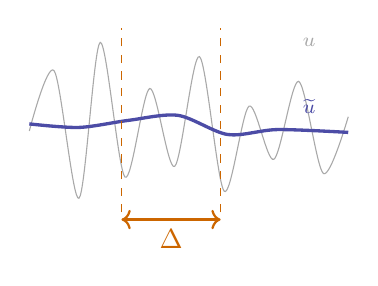
\begin{tikzpicture}[x=0.9cm,y=0.9cm]
  \draw[modelgray,thin] plot[smooth] coordinates{(0,1.4)(0.35,2.25)(0.7,0.45)(1.0,2.65)(1.35,0.75)(1.7,2.0)(2.05,0.9)(2.4,2.45)(2.75,0.55)(3.1,1.75)(3.45,1.0)(3.8,2.1)(4.15,0.8)(4.5,1.6)};
  \draw[modelblue,very thick] plot[smooth] coordinates{(0,1.5)(0.7,1.45)(1.4,1.55)(2.1,1.62)(2.8,1.35)(3.5,1.42)(4.5,1.38)};
  \draw[<->,modelorange,thick] (1.3,0.15)--(2.7,0.15) node[midway,below]{$\Delta$};
  \draw[dashed,modelorange] (1.3,0.25)--(1.3,2.85);
  \draw[dashed,modelorange] (2.7,0.25)--(2.7,2.85);
  \node[modelgray] at (3.95,2.65){\scriptsize $u$};
  \node[modelblue] at (3.95,1.75){\scriptsize $\widetilde u$};
\end{tikzpicture}
\end{column}
\end{columns}
\end{frame}

% ----- 20. Filtered equations -----
\begin{frame}{Filtering the nonlinearity creates SGS stress}
Assuming a homogeneous filter that commutes with differentiation,
\begin{align*}
  \partial_t\widetilde u_i+\widetilde u_j\partial_j\widetilde u_i
  &= -\partial_i\widetilde p+\nu\partial_{jj}\widetilde u_i
     -\partial_j\tau_{ij},\\
  \partial_i\widetilde u_i&=0,
\end{align*}
with
\[
  \boxed{\tau_{ij}:=\widetilde{u_iu_j}-\widetilde u_i\widetilde u_j.}
\]

\begin{punchbox}
There is no need to assert a unique additive ``subgrid velocity.'' The exact closure term is the difference between a filtered product and the product of filtered fields.
\end{punchbox}
\end{frame}

% ----- 21. Filter width -----
\begin{frame}{The LES cutoff is tied to grid and numerics}
\begin{columns}[T,onlytextwidth]
\begin{column}{0.54\textwidth}
In an explicit-filter view, $G_\Delta$ defines the cutoff. In many practical LES calculations, the discretization supplies an \emph{effective} filter.

\begin{itemize}\itemsep4pt
  \item Variable filter width and boundaries can make filtering and differentiation fail to commute.
  \item A nominal SGS model cannot compensate for an under-resolved, overly dissipative, or dispersive scheme in every regime.
  \item Report $\Delta$, mesh anisotropy, and numerical method with the closure.
\end{itemize}
\end{column}
\begin{column}{0.43\textwidth}
\centering
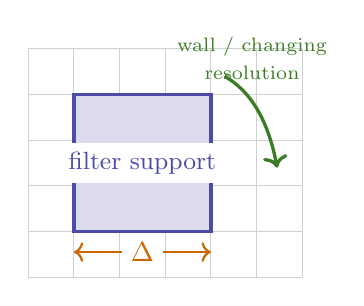
\begin{tikzpicture}[x=0.58cm,y=0.58cm]
  \foreach \i in {0,...,6}{\draw[modelgray!55] (\i,0) -- (\i,5);}
  \foreach \j in {0,...,5}{\draw[modelgray!55] (0,\j) -- (6,\j);}
  \fill[modelblue!20] (1,1) rectangle (4,4);
  \draw[modelblue,very thick] (1,1) rectangle (4,4);
  \node[modelblue,fill=white] at (2.5,2.5){\small filter support};
  \draw[<->,modelorange,thick] (1,0.55)--(4,0.55) node[midway,fill=white]{$\Delta$};
  \draw[modelgreen,very thick,->] (4.3,4.4) .. controls (5.0,4.0) and (5.3,3.2) .. (5.45,2.4);
  \node[modelgreen,align=center] at (4.9,4.8){\scriptsize wall / changing\\[-2pt]\scriptsize resolution};
\end{tikzpicture}
\end{column}
\end{columns}
\end{frame}

% ----- 22. Smagorinsky -----
\begin{frame}{Smagorinsky closes the deviatoric SGS stress}
The eddy-viscosity SGS hypothesis is
\[
  \tau_{ij}^{\mathrm{dev}}=-2\nu_{\mathrm{sgs}}\widetilde S_{ij},
  \qquad
  \widetilde S_{ij}=\tfrac12(\partial_j\widetilde u_i+\partial_i\widetilde u_j).
\]
The classical Smagorinsky model sets
\[
  \nu_{\mathrm{sgs}}=(C_s\Delta)^2|\widetilde S|,
  \qquad
  |\widetilde S|=\sqrt{2\widetilde S_{ij}\widetilde S_{ij}}.
\]
{\small $C_s\approx0.17$ for isotropic turbulence (Lilly), reduced to $\approx0.1$ in shear flows.}
{\scriptsize\soft{(Lilly 1967 obtained $C_s\approx0.17$ by matching the mean SGS dissipation to a Kolmogorov inertial range with $C_K\approx1.5$; Deardorff 1970 found $\approx0.1$ necessary in channel flow, where mean shear adds to $|\widetilde S|$.)}\par}

\begin{columns}[T,onlytextwidth]
\begin{column}{0.52\textwidth}
For $\nu_{\mathrm{sgs}}\ge0$, the modeled transfer is
\[
  \Pi=-\tau_{ij}\widetilde S_{ij}
  =2\nu_{\mathrm{sgs}}\widetilde S_{ij}\widetilde S_{ij}\ge0.
\]
{\scriptsize The isotropic part of $\tau_{ij}$ drops out because $\widetilde S_{ii}=0$.\par}
\end{column}
\begin{column}{0.44\textwidth}
\begin{alertblock}{Consequence}
The basic model is purely dissipative and needs wall damping or a dynamic treatment near walls.
\end{alertblock}
\end{column}
\end{columns}
\end{frame}

% ----- 23. Dynamic procedure -----
\begin{frame}{The Germano procedure estimates coefficients from resolved scales}
\begin{columns}[T,onlytextwidth]
\begin{column}{0.55\textwidth}
Apply a second, wider \emph{test filter} $\widehat{(\cdot)}$ and use the identity
\[
  L_{ij}=T_{ij}-\widehat{\tau}_{ij}
  =\widehat{\widetilde u_i\widetilde u_j}
   -\widehat{\widetilde u}_i\widehat{\widetilde u}_j.
\]
{\small Here $T_{ij}:=\widehat{\widetilde{u_iu_j}}-\widehat{\widetilde u}_i\widehat{\widetilde u}_j$ is the stress at the combined (grid then test) filter level. $L_{ij}$ is computable from the resolved field alone.\par}
A modeled form on both filter levels gives an equation for a local or averaged coefficient.

\begin{itemize}\itemsep0pt
  \item adapts to flow and resolution;
  \item clipping/averaging is often used for robustness;
  \item local backscatter can occur when the inferred coefficient is negative.
\end{itemize}
\end{column}
\begin{column}{0.42\textwidth}
\centering
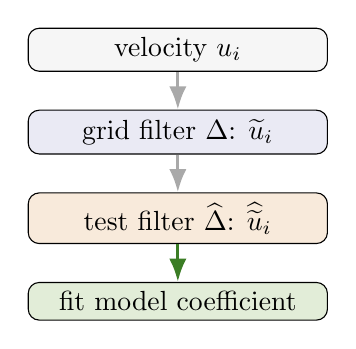
\begin{tikzpicture}[node distance=0.48cm,>=Latex]
  \node[draw,rounded corners,fill=modelgray!10,minimum width=3.8cm] (raw) {velocity $u_i$};
  \node[draw,rounded corners,fill=modelblue!12,below=of raw,minimum width=3.8cm] (grid) {grid filter $\Delta$: $\widetilde u_i$};
  \node[draw,rounded corners,fill=modelorange!14,below=of grid,minimum width=3.8cm] (test) {test filter $\widehat\Delta$: $\widehat{\widetilde u}_i$};
  \node[draw,rounded corners,fill=modelgreen!12,below=of test,minimum width=3.8cm] (coef) {fit model coefficient};
  \draw[->,very thick,modelgray] (raw)--(grid);
  \draw[->,very thick,modelgray] (grid)--(test);
  \draw[->,very thick,modelgreen] (test)--(coef);
\end{tikzpicture}
\end{column}
\end{columns}
\end{frame}

% ----- 24. Cascade -----
\begin{frame}{The spectral picture motivates---but does not prove---eddy viscosity}
\begin{columns}[T,onlytextwidth]
\begin{column}{0.52\textwidth}
In three-dimensional turbulence, kinetic energy transfers toward smaller scales \emph{on average} through the inertial range and is dissipated near the Kolmogorov scale.

\begin{itemize}\itemsep4pt
  \item LES resolves $k\lesssim k_c$ (length scales $\gtrsim\Delta$); adequate numerical resolution is still required.
  \item SGS models represent net transfer through that cutoff.
  \item Instantaneous, local transfer can be upscale (backscatter).
\end{itemize}

\soft{The $-5/3$ spectrum is an inertial-range idealization, not a guarantee in every finite, anisotropic flow.}
\end{column}
\begin{column}{0.45\textwidth}
\centering
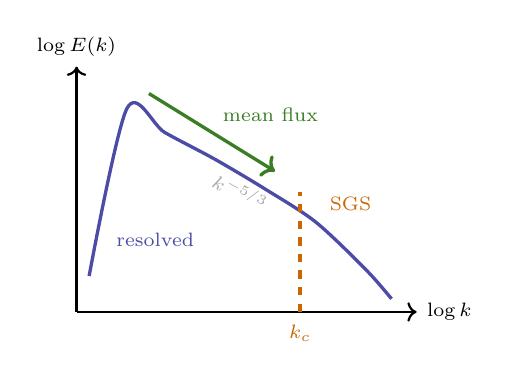
\begin{tikzpicture}[x=0.8cm,y=0.76cm]
  \draw[->,thick] (0,0)--(5.4,0) node[right]{\scriptsize $\log k$};
  \draw[->,thick] (0,0)--(0,4.1) node[above]{\scriptsize $\log E(k)$};
  \draw[modelblue,very thick] plot[smooth] coordinates{(0.2,0.6)(0.8,3.4)(1.4,3.0)(2.2,2.55)(3.0,2.05)(3.8,1.5)(4.6,0.7)(5.0,0.22)};
  \draw[dashed,modelorange,very thick] (3.55,0)--(3.55,2.0);
  \node[modelorange] at (3.55,-0.35){\scriptsize $k_c$};
  \draw[->,modelgreen,very thick] (1.15,3.65)--(3.15,2.35) node[midway,above right]{\scriptsize mean flux};
  \node[modelblue] at (1.25,1.2){\scriptsize resolved};
  \node[modelorange] at (4.35,1.8){\scriptsize SGS};
  \node[rotate=-29,modelgray] at (2.6,2.0){\scriptsize $k^{-5/3}$};
\end{tikzpicture}
\end{column}
\end{columns}
\end{frame}

% ----- 25. LES vs RANS -----
\begin{frame}{LES versus RANS: compare requirements, not slogans}
\small
\begin{tabular}{@{}L{0.27\textwidth}L{0.32\textwidth}L{0.34\textwidth}@{}}
\toprule
& \textbf{RANS/URANS} & \textbf{LES}\\
\midrule
Primary output & mean or phase-resolved mean & filtered unsteady field plus statistics\\[3pt]
Closure target & Reynolds stress $R_{ij}$ & SGS stress $\tau_{ij}$\\[3pt]
Grid demand & resolve mean gradients and wall treatment & resolve energy-containing eddies; wall-resolved demand grows steeply with $\Rey$\\[3pt]
Strength & economical design calculations & unsteady structures, mixing, wakes\\[3pt]
Risk & closure bias in nonequilibrium flow & grid/numerics/inflow/wall-model dependence\\
\bottomrule
\end{tabular}

\vspace{0.55em}
\begin{punchbox}
LES is not generically ``more accurate.'' Its advantage is conditional on resolving the motions that control the target quantity.
\end{punchbox}
\end{frame}

% ----- 26. Wind farm -----
\begin{frame}{Application: LES can expose interacting turbine wakes}
\begin{columns}[T,onlytextwidth]
\begin{column}{0.48\textwidth}
Wind-farm calculations illustrate why resolved unsteadiness matters:
\begin{itemize}\itemsep4pt
  \item atmospheric turbulence enters the array;
  \item rotating turbines extract momentum;
  \item wakes expand, meander, and merge;
  \item downstream power and loading depend on recovery.
\end{itemize}

\soft{The turbine and near-wall physics may still require actuator and wall models.}
\end{column}
\begin{column}{0.49\textwidth}
\centering
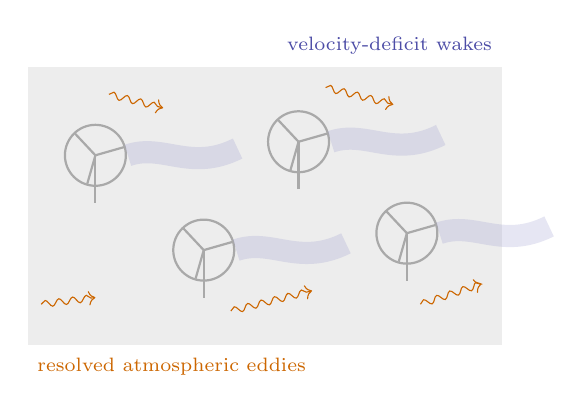
\begin{tikzpicture}[x=0.86cm,y=0.86cm]
  \fill[LightGray!40] (0,0) rectangle (7.0,4.1);
  \foreach \x/\y in {1.0/2.8,2.6/1.4,4.0/3.0,5.6/1.65}{
    \draw[modelgray,thick] (\x,\y-0.7)--(\x,\y);
    \draw[modelgray,thick] (\x,\y) circle (0.45);
    \draw[modelgray,thick] (\x,\y)--(\x+0.42,\y+0.12);
    \draw[modelgray,thick] (\x,\y)--(\x-0.12,\y-0.42);
    \draw[modelgray,thick] (\x,\y)--(\x-0.30,\y+0.32);
    \draw[modelblue!55,line width=8pt,opacity=0.25] (\x+0.48,\y) .. controls (\x+1.0,\y+0.18) and (\x+1.4,\y-0.25) .. (\x+2.1,\y+0.1);
  }
  \foreach \a/\b/\c/\d in {0.2/0.6/1.0/0.7,1.2/3.7/2.0/3.5,3.0/0.5/4.2/0.8,4.4/3.8/5.4/3.55,5.8/0.6/6.7/0.9}{
    \draw[decorate,decoration={snake,amplitude=1.2pt,segment length=5pt},modelorange,->] (\a,\b)--(\c,\d);
  }
  \node[modelblue,anchor=south east] at (7.0,4.15){\scriptsize velocity-deficit wakes};
  \node[modelorange,anchor=north west] at (0,-0.05){\scriptsize resolved atmospheric eddies};
\end{tikzpicture}
\end{column}
\end{columns}
\end{frame}

% ----- 27. DES -----
\begin{frame}{Hybrid RANS--LES partitions modeled and resolved regions}
\begin{columns}[T,onlytextwidth]
\begin{column}{0.52\textwidth}
Detached-Eddy Simulation (DES) was introduced as an SA-based method that uses a grid-sensitive length scale:
\begin{itemize}\itemsep4pt
  \item RANS-like behavior in attached near-wall layers;
  \item LES-like behavior where the grid supports separated eddies.
\end{itemize}

It is not a sharp switch based only on ``steady'' versus ``unsteady'' flow. Grid-induced separation and modeled-stress depletion motivated shielding strategies such as DDES.
\end{column}
\begin{column}{0.45\textwidth}
\centering
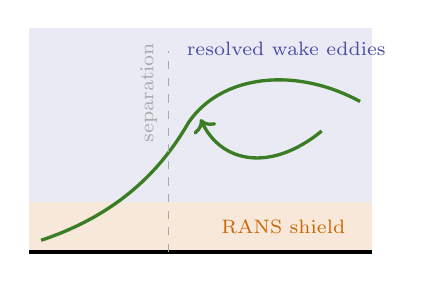
\begin{tikzpicture}[x=0.75cm,y=0.75cm]
  \fill[modelorange!15] (0,0) rectangle (5.8,0.85);
  \fill[modelblue!12] (0,0.85) rectangle (5.8,3.8);
  \draw[very thick] (0,0)--(5.8,0);
  \draw[modelgreen,very thick] (0.2,0.2) .. controls (1.7,0.7) and (2.35,1.6) .. (2.7,2.2)
    .. controls (3.25,3.0) and (4.5,3.15) .. (5.6,2.55);
  \draw[modelgreen,very thick,->] (4.95,2.05) .. controls (4.1,1.35) and (3.25,1.5) .. (2.9,2.25);
  \node[modelorange] at (4.3,0.43){\scriptsize RANS shield};
  \node[modelblue] at (4.35,3.45){\scriptsize resolved wake eddies};
  \draw[dashed,modelgray] (2.35,0)--(2.35,3.4);
  \node[rotate=90,modelgray,anchor=south] at (2.33,2.7){\scriptsize separation};
\end{tikzpicture}
\end{column}
\end{columns}
\end{frame}

% ----- 28. ML -----
\begin{frame}{Machine-learned closure must survive the solver loop}
\centering
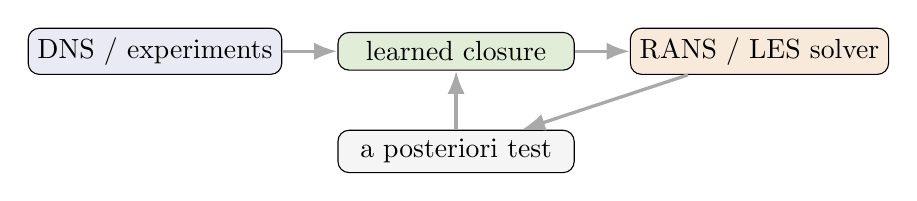
\begin{tikzpicture}[node distance=0.7cm,>=Latex]
  \node[draw,rounded corners,fill=modelblue!12,minimum width=3.0cm] (data) {DNS / experiments};
  \node[draw,rounded corners,fill=modelgreen!12,right=of data,minimum width=3.0cm] (fit) {learned closure};
  \node[draw,rounded corners,fill=modelorange!14,right=of fit,minimum width=3.0cm] (solver) {RANS / LES solver};
  \node[draw,rounded corners,fill=modelgray!12,below=0.75cm of fit,minimum width=3.0cm] (test) {a posteriori test};
  \draw[->,very thick,modelgray] (data)--(fit);
  \draw[->,very thick,modelgray] (fit)--(solver);
  \draw[->,very thick,modelgray] (solver)--(test);
  \draw[->,very thick,modelgray] (test)--(fit);
\end{tikzpicture}

\vspace{0.65em}
Useful training accuracy is not sufficient. A closure should respect relevant
\begin{itemize}\itemsep3pt
  \item symmetries/invariance and dimensional consistency;
  \item realizability and appropriate energy transfer;
  \item numerical stability and out-of-distribution behavior;
  \item coupled, \emph{a posteriori} performance in the PDE solver.
\end{itemize}
\end{frame}

% ----- 29. Summary -----
\begin{frame}{A closure decision tree}
\centering
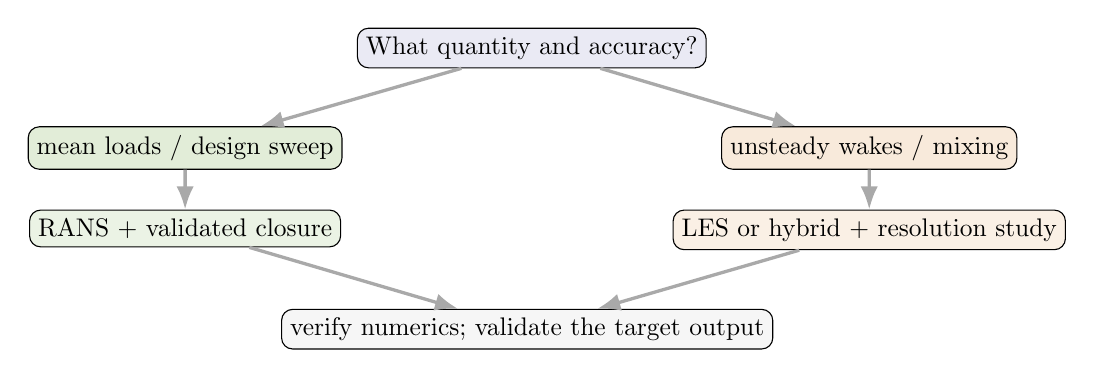
\begin{tikzpicture}[scale=0.92,transform shape,node distance=0.55cm and 0.65cm,>=Latex]
  \node[draw,rounded corners,fill=modelblue!12,minimum width=3.4cm] (qoi) {What quantity and accuracy?};
  \node[draw,rounded corners,fill=modelgreen!12,below left=0.8cm and 0.2cm of qoi,minimum width=3.2cm] (mean) {mean loads / design sweep};
  \node[draw,rounded corners,fill=modelorange!14,below right=0.8cm and 0.2cm of qoi,minimum width=3.2cm] (unsteady) {unsteady wakes / mixing};
  \node[draw,rounded corners,fill=modelgreen!8,below=of mean,minimum width=3.2cm] (rans) {RANS + validated closure};
  \node[draw,rounded corners,fill=modelorange!10,below=of unsteady,minimum width=3.2cm] (les) {LES or hybrid + resolution study};
  \node[draw,rounded corners,fill=modelgray!10,below=1.1cm of $(rans)!0.5!(les)$,minimum width=5.4cm] (verify) {verify numerics; validate the target output};
  \draw[->,very thick,modelgray] (qoi)--(mean);
  \draw[->,very thick,modelgray] (qoi)--(unsteady);
  \draw[->,very thick,modelgray] (mean)--(rans);
  \draw[->,very thick,modelgray] (unsteady)--(les);
  \draw[->,very thick,modelgray] (rans)--(verify);
  \draw[->,very thick,modelgray] (les)--(verify);
\end{tikzpicture}

\vspace{0.65em}
\begin{punchbox}
\centering
RANS averages; LES filters. Both create exact unresolved stresses, and every practical closure carries assumptions that must be tested in the intended regime.
\end{punchbox}
\end{frame}

% ----- 30. References -----
\begin{frame}{Primary sources and durable resources}
\footnotesize
\begin{itemize}\itemsep4pt
  \item J. Smagorinsky, ``General circulation experiments with the primitive equations. I. The basic experiment,'' \emph{Monthly Weather Review} 91 (1963), 99--164. \href{https://doi.org/10.1175/1520-0493(1963)091\%3C0099:GCEWTP\%3E2.3.CO;2}{\texttt{doi:10.1175/1520-0493(1963)091\textless{}0099:GCEWTP\textgreater{}2.3.CO;2}}.
  \item M. Germano, U. Piomelli, P. Moin, and W. H. Cabot, ``A dynamic subgrid-scale eddy viscosity model,'' \emph{Physics of Fluids A} 3 (1991), 1760--1765. \href{https://doi.org/10.1063/1.857955}{doi:10.1063/1.857955}.
  \item P. R. Spalart and S. R. Allmaras, ``A one-equation turbulence model for aerodynamic flows,'' AIAA Paper 92-0439 (1992). \href{https://doi.org/10.2514/6.1992-439}{doi:10.2514/6.1992-439}.
  \item P. R. Spalart, W.-H. Jou, M. Strelets, and S. R. Allmaras, ``Comments on the feasibility of LES for wings, and on a hybrid RANS/LES approach,'' Advances in DNS/LES (1997).
  \item NASA Langley Turbulence Modeling Resource: \href{https://tmbwg.github.io/turbmodels/}{tmbwg.github.io/turbmodels/} (equations, variants, and verification cases).
  \item Adapted in part from educational material by Steven L. Brunton.
\end{itemize}
\end{frame}

% ----- 30b. References, continued -----
\begin{frame}{Primary sources and durable resources (continued)}
\scriptsize
\begin{itemize}\itemsep3pt
  \item S. B. Pope, \emph{Turbulent Flows}, Cambridge University Press (2000): Ch.~4--5 (RANS, TKE budget, pseudo-dissipation), Ch.~7 (wall units, log law), Ch.~10 (eddy-viscosity and two-equation models), Ch.~13 (LES, Smagorinsky, dynamic model).
  \item D. C. Wilcox, \emph{Turbulence Modeling for CFD}, 3rd ed., DCW Industries (2006).
  \item D. C. Wilcox, ``Reassessment of the scale-determining equation for advanced turbulence models,'' \emph{AIAA J.} 26 (1988), 1299--1310. \href{https://doi.org/10.2514/3.10041}{doi:10.2514/3.10041}.
  \item B. E. Launder and D. B. Spalding, ``The numerical computation of turbulent flows,'' \emph{Comput. Methods Appl. Mech. Eng.} 3 (1974), 269--289. \href{https://doi.org/10.1016/0045-7825(74)90029-2}{doi:10.1016/0045-7825(74)90029-2}.
  \item F. R. Menter, ``Two-equation eddy-viscosity turbulence models for engineering applications,'' \emph{AIAA J.} 32 (1994), 1598--1605. \href{https://doi.org/10.2514/3.12149}{doi:10.2514/3.12149}.
  \item D. K. Lilly, ``The representation of small-scale turbulence in numerical simulation experiments,'' \emph{Proc. IBM Scientific Computing Symposium on Environmental Sciences} (1967), 195--210.
  \item J. W. Deardorff, ``A numerical study of three-dimensional turbulent channel flow at large Reynolds numbers,'' \emph{J. Fluid Mech.} 41 (1970), 453--480. \href{https://doi.org/10.1017/S0022112070000691}{doi:10.1017/S0022112070000691}.
  \item P. R. Spalart, S. Deck, M. L. Shur, K. D. Squires, M. Kh. Strelets, and A. Travin, ``A new version of detached-eddy simulation, resistant to ambiguous grid densities,'' \emph{Theor. Comput. Fluid Dyn.} 20 (2006), 181--195. \href{https://doi.org/10.1007/s00162-006-0015-0}{doi:10.1007/s00162-006-0015-0}.
  \item All schematics in this deck: instructor's course notes.
\end{itemize}
\end{frame}

\end{document}
